\hypertarget{SurrogateSplits_8c}{
\section{Surrogate\-Splits.c File Reference}
\label{SurrogateSplits_8c}\index{SurrogateSplits.c@{SurrogateSplits.c}}
}
{\tt \#include \char`\"{}party.h\char`\"{}}\par


Include dependency graph for Surrogate\-Splits.c:\begin{figure}[H]
\begin{center}
\leavevmode
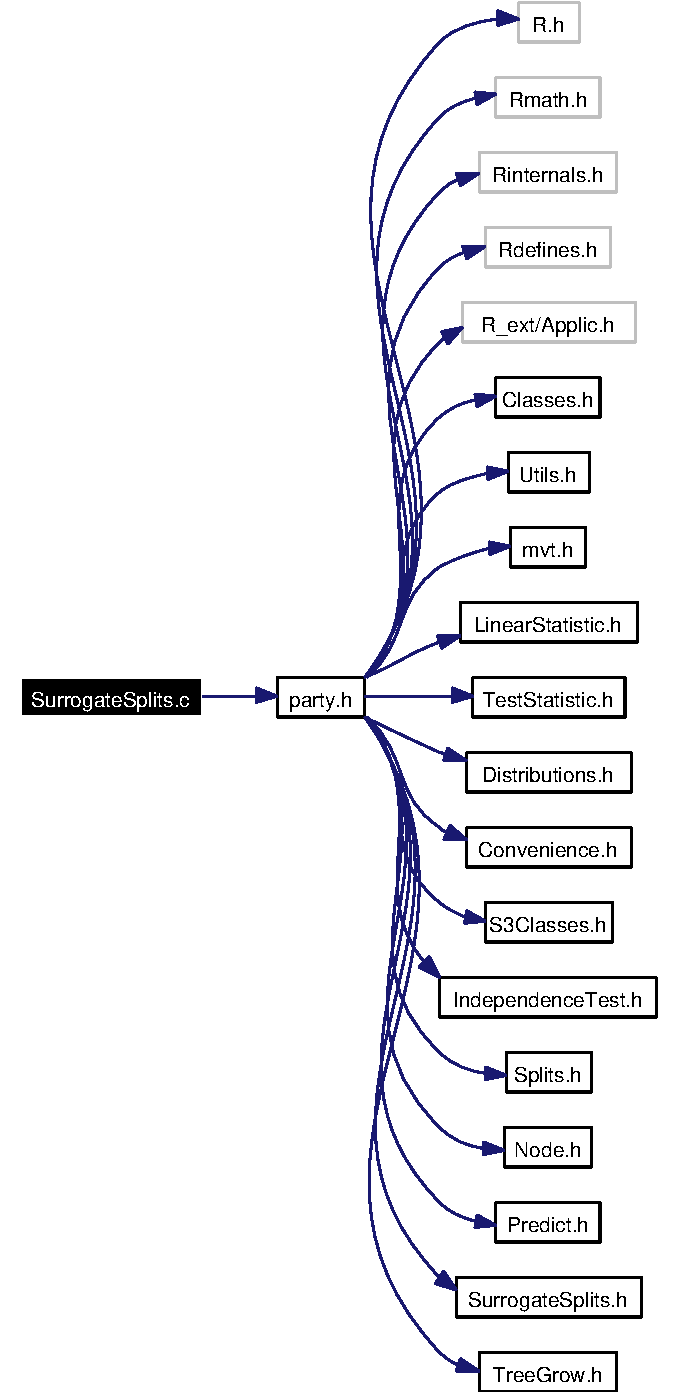
\includegraphics[width=179pt]{SurrogateSplits_8c__incl}
\end{center}
\end{figure}
\subsection*{Functions}
\begin{CompactItemize}
\item 
void \hyperlink{SurrogateSplits_8c_a0}{C\_\-surrogates} (SEXP node, SEXP learnsample, SEXP weights, SEXP controls, SEXP fitmem)
\item 
SEXP \hyperlink{SurrogateSplits_8c_a1}{R\_\-surrogates} (SEXP node, SEXP learnsample, SEXP weights, SEXP controls, SEXP fitmem)
\item 
void \hyperlink{SurrogateSplits_8c_a2}{C\_\-splitsurrogate} (SEXP node, SEXP learnsample)
\end{CompactItemize}


\subsection{Detailed Description}
Suggorgate splits

\begin{Desc}
\item[Author:]\begin{Desc}
\item[Author]hothorn \end{Desc}
\end{Desc}
\begin{Desc}
\item[Date:]\begin{Desc}
\item[Date]2006-08-25 10:53:10 +0200 (Fri, 25 Aug 2006) \end{Desc}
\end{Desc}


Definition in file \hyperlink{SurrogateSplits_8c-source}{Surrogate\-Splits.c}.

\subsection{Function Documentation}
\hypertarget{SurrogateSplits_8c_a2}{
\index{SurrogateSplits.c@{Surrogate\-Splits.c}!C_splitsurrogate@{C\_\-splitsurrogate}}
\index{C_splitsurrogate@{C\_\-splitsurrogate}!SurrogateSplits.c@{Surrogate\-Splits.c}}
\subsubsection[C\_\-splitsurrogate]{\setlength{\rightskip}{0pt plus 5cm}void C\_\-splitsurrogate (SEXP {\em node}, SEXP {\em learnsample})}}
\label{SurrogateSplits_8c_a2}


Split with missing values \par
 \begin{Desc}
\item[Parameters:]
\begin{description}
\item[{\em node}]the current node with primary and surrogate splits specified \item[{\em learnsample}]learning sample\end{description}
\end{Desc}


Definition at line 169 of file Surrogate\-Splits.c.

References get\_\-missings(), get\_\-nobs(), get\_\-variable(), has\_\-missings(), PL2\_\-inputs\-Sym, S3get\_\-leftnode(), S3get\_\-nodeweights(), S3get\_\-primarysplit(), S3get\_\-rightnode(), S3get\_\-splitpoint(), S3get\_\-surrogatesplits(), S3get\_\-toleft(), and S3get\_\-variable\-ID().

Referenced by C\_\-Tree\-Grow().

Here is the call graph for this function:\begin{figure}[H]
\begin{center}
\leavevmode
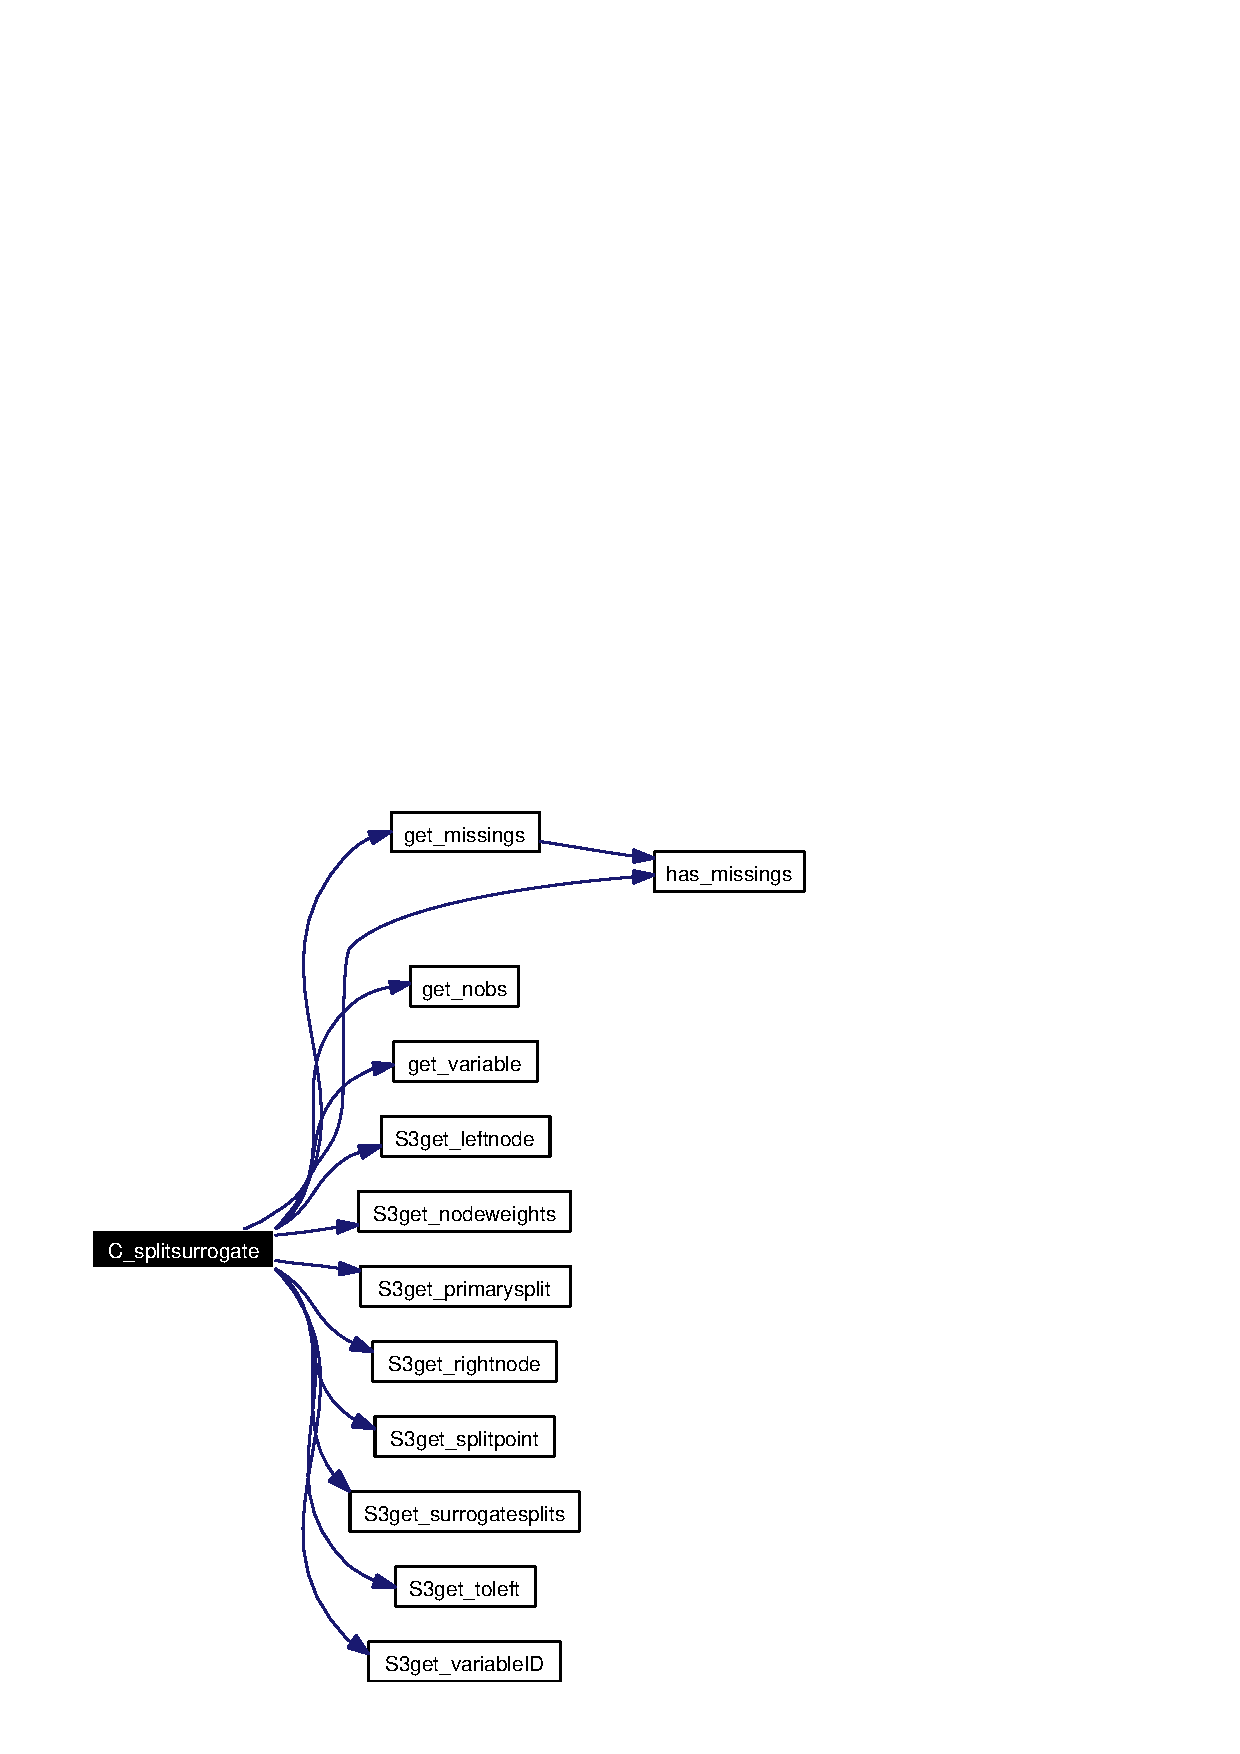
\includegraphics[width=195pt]{SurrogateSplits_8c_a2_cgraph}
\end{center}
\end{figure}
\hypertarget{SurrogateSplits_8c_a0}{
\index{SurrogateSplits.c@{Surrogate\-Splits.c}!C_surrogates@{C\_\-surrogates}}
\index{C_surrogates@{C\_\-surrogates}!SurrogateSplits.c@{Surrogate\-Splits.c}}
\subsubsection[C\_\-surrogates]{\setlength{\rightskip}{0pt plus 5cm}void C\_\-surrogates (SEXP {\em node}, SEXP {\em learnsample}, SEXP {\em weights}, SEXP {\em controls}, SEXP {\em fitmem})}}
\label{SurrogateSplits_8c_a0}


Search for surrogate splits for bypassing the primary split \par
 \begin{Desc}
\item[Parameters:]
\begin{description}
\item[{\em node}]the current node with primary split specified \item[{\em learnsample}]learning sample \item[{\em weights}]the weights associated with the current node \item[{\em controls}]an object of class `Tree\-Control' \item[{\em fitmem}]an object of class `Tree\-Fit\-Memory' \end{description}
\end{Desc}
\begin{Desc}
\item[\hyperlink{todo__todo000003}{Todo}]enable nominal surrogate split variables as well \end{Desc}


Definition at line 21 of file Surrogate\-Splits.c.

References C\_\-Expect\-Covar\-Influence(), C\_\-init\_\-orderedsplit(), C\_\-split(), get\_\-maxsurrogate(), get\_\-missings(), get\_\-ninputs(), get\_\-nobs(), get\_\-ordering(), get\_\-splitctrl(), get\_\-splitstatistics(), get\_\-variable(), get\_\-weights(), has\_\-missings(), is\_\-nominal(), PL2\_\-expcovinfss\-Sym, PL2\_\-inputs\-Sym, PL2\_\-linexpcov2sample\-Sym, S3get\_\-nodeweights(), S3get\_\-primarysplit(), S3get\_\-splitpoint(), S3get\_\-surrogatesplits(), S3get\_\-variable\-ID(), S3set\_\-toleft(), S3set\_\-variable\-ID(), and SPLIT\_\-LENGTH.

Referenced by C\_\-Tree\-Grow(), and R\_\-surrogates().

Here is the call graph for this function:\begin{figure}[H]
\begin{center}
\leavevmode
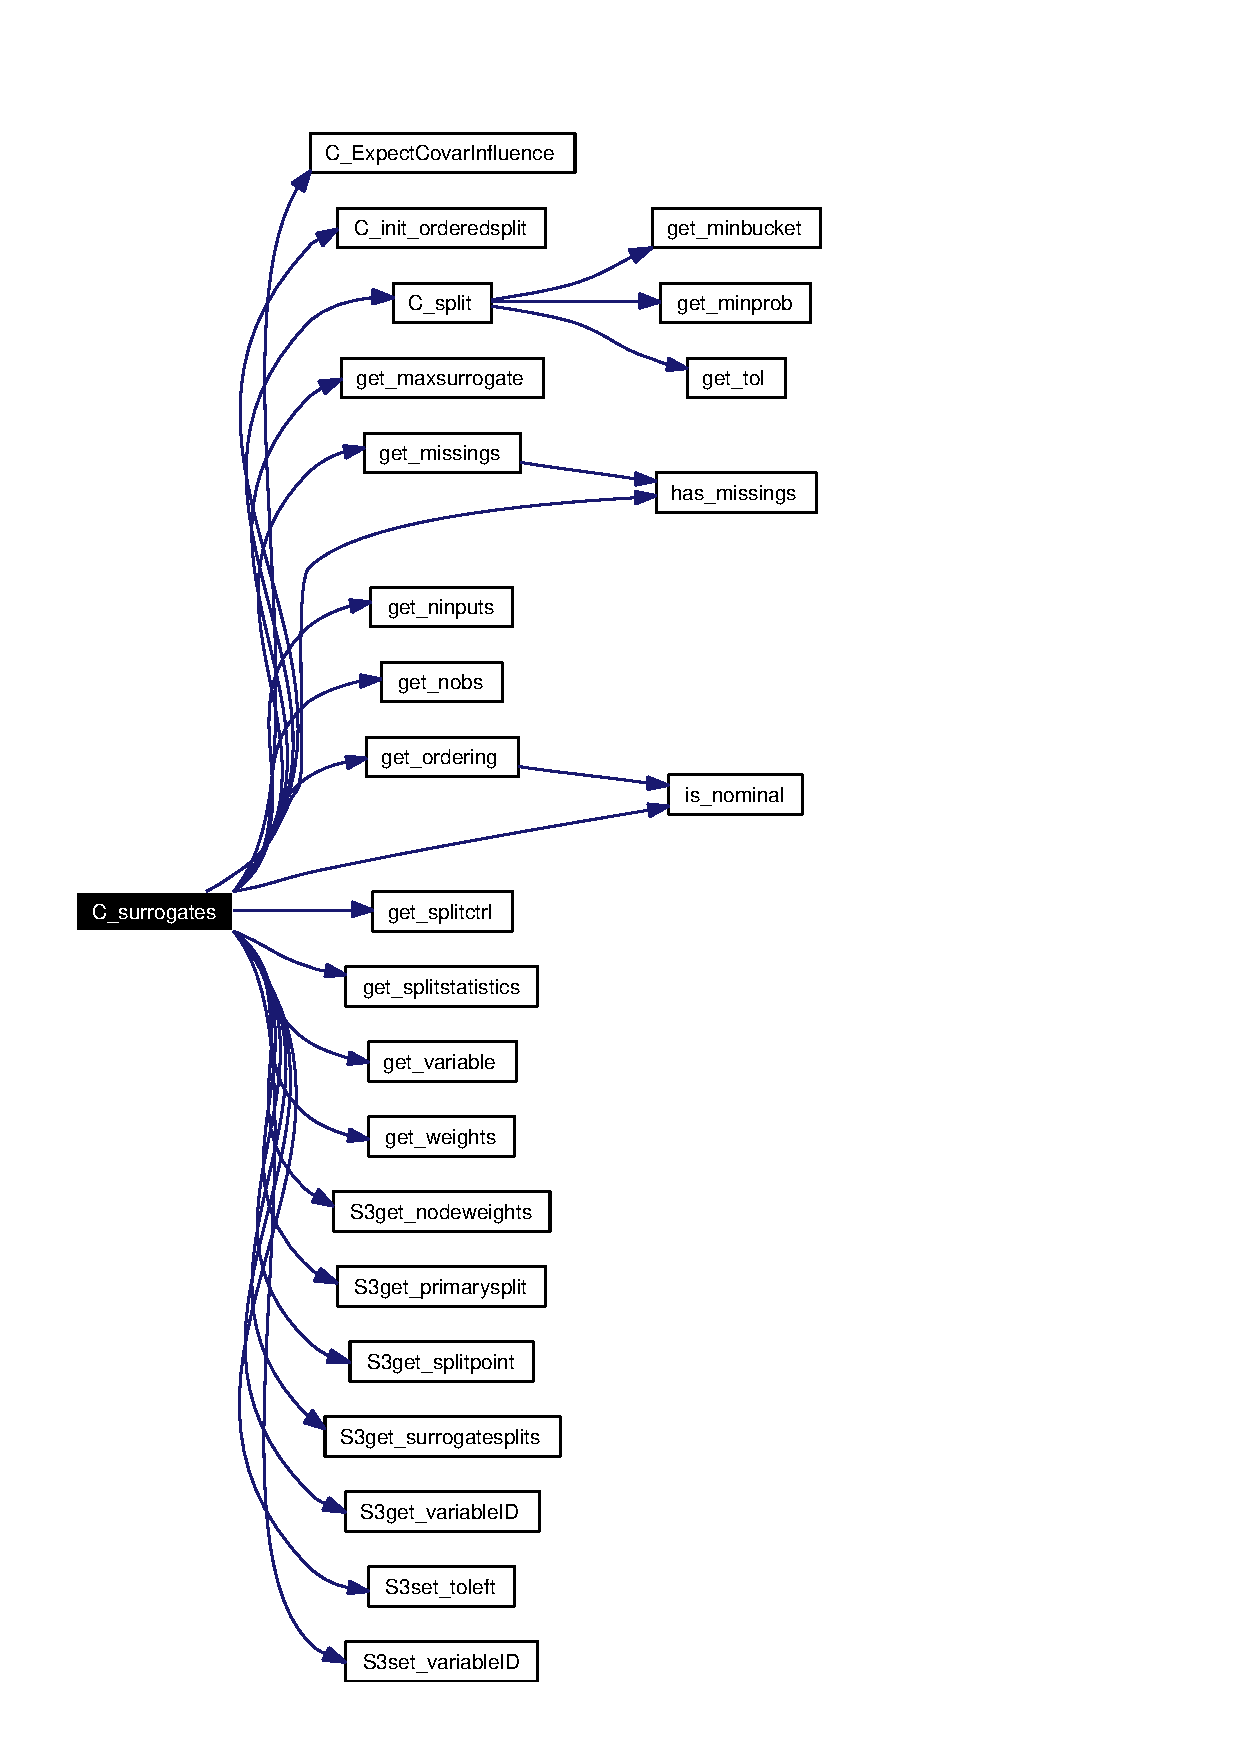
\includegraphics[width=197pt]{SurrogateSplits_8c_a0_cgraph}
\end{center}
\end{figure}
\hypertarget{SurrogateSplits_8c_a1}{
\index{SurrogateSplits.c@{Surrogate\-Splits.c}!R_surrogates@{R\_\-surrogates}}
\index{R_surrogates@{R\_\-surrogates}!SurrogateSplits.c@{Surrogate\-Splits.c}}
\subsubsection[R\_\-surrogates]{\setlength{\rightskip}{0pt plus 5cm}SEXP R\_\-surrogates (SEXP {\em node}, SEXP {\em learnsample}, SEXP {\em weights}, SEXP {\em controls}, SEXP {\em fitmem})}}
\label{SurrogateSplits_8c_a1}


R-interface to C\_\-surrogates \par
 \begin{Desc}
\item[Parameters:]
\begin{description}
\item[{\em node}]the current node with primary split specified \item[{\em learnsample}]learning sample \item[{\em weights}]the weights associated with the current node \item[{\em controls}]an object of class `Tree\-Control' \item[{\em fitmem}]an object of class `Tree\-Fit\-Memory'\end{description}
\end{Desc}


Definition at line 154 of file Surrogate\-Splits.c.

References C\_\-surrogates(), and S3get\_\-surrogatesplits().

Here is the call graph for this function:\begin{figure}[H]
\begin{center}
\leavevmode
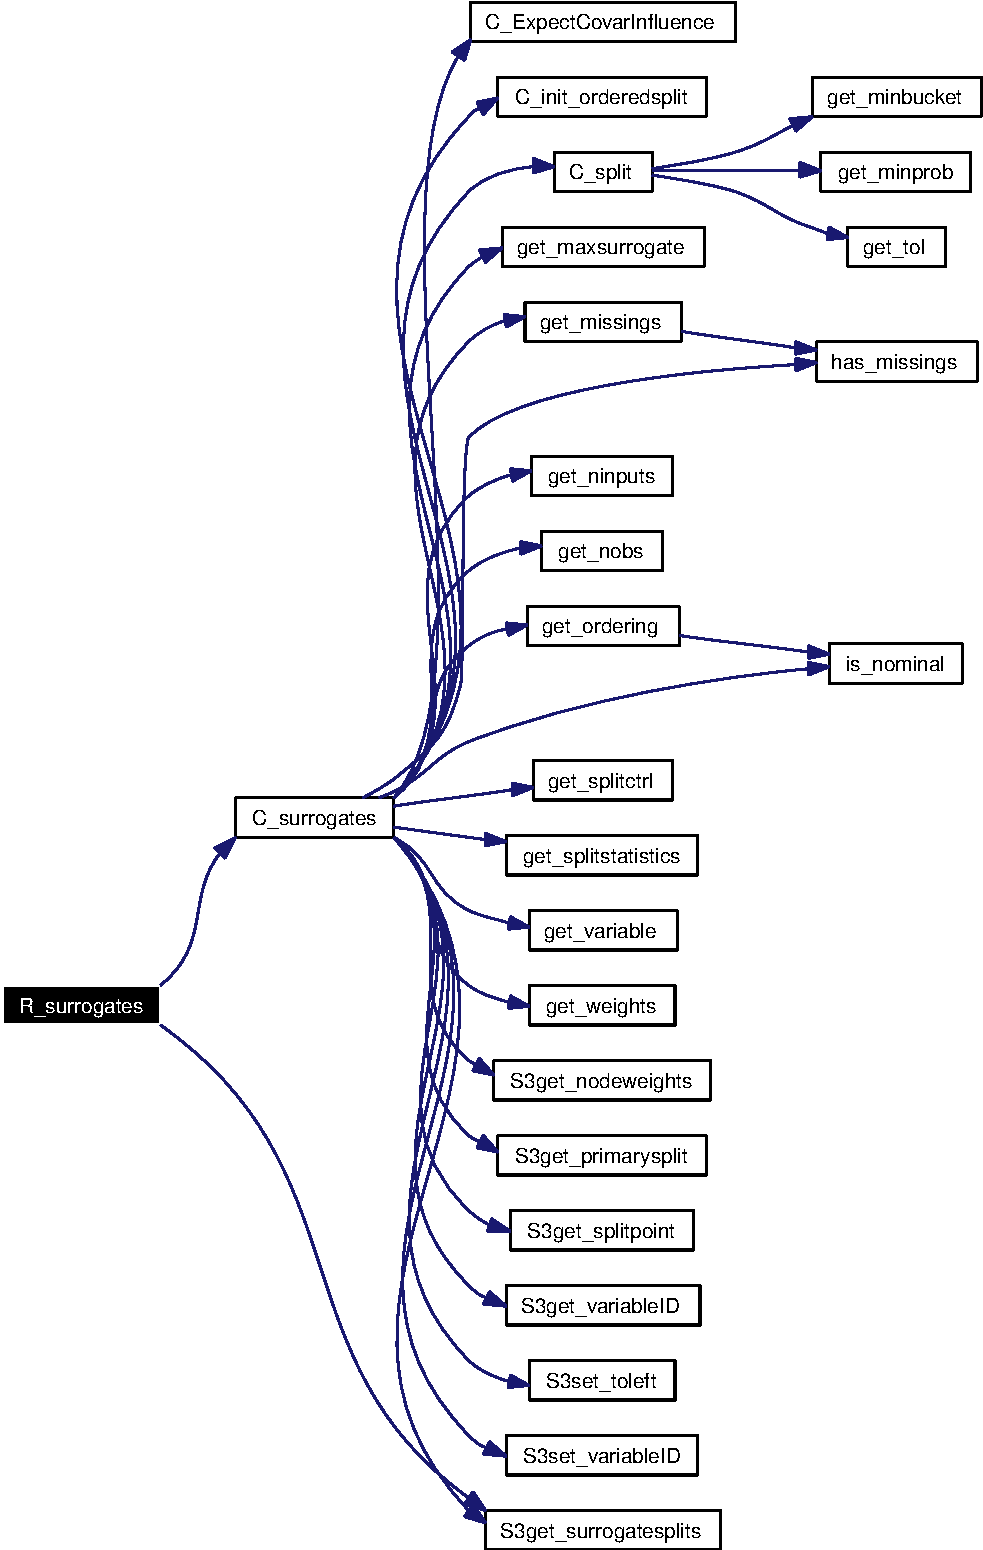
\includegraphics[width=253pt]{SurrogateSplits_8c_a1_cgraph}
\end{center}
\end{figure}
